% ------------------------------------------------------------------------------
% TYPO3 Version 10.3 - What's New (German Version)
%
% @license	Creative Commons BY-NC-SA 3.0
% @link		https://typo3.org/help/documentation/whats-new/
% @language	German
% ------------------------------------------------------------------------------

\section{Änderungen für Integratoren}
\begin{frame}[fragile]
	\frametitle{Änderungen für Integratoren}

	\begin{center}\huge{Kapitel 2:}\end{center}
	\begin{center}\huge{\color{typo3darkgrey}\textbf{Änderungen für Integratoren}}\end{center}

\end{frame}

% ------------------------------------------------------------------------------
% Feature | 90333 | Dashboard

\begin{frame}[fragile]
	\frametitle{Änderungen für Integratoren}
	\framesubtitle{Dashboard}

	% decrease font size for code listing
	\lstset{basicstyle=\tiny\ttfamily}

	\begin{itemize}
		\item Dashboard \textit{presets} können für neue Benutzer oder für Benutzer, die alle ihre Dashboards gelöscht haben, konfiguriert werden.
		\item Dies kann verwendet werden, um ein "Getting Started"-Dashboard standardmäßig anzuzeigen.
		\item Eine TSconfig ist dann zum Beispiel:

\vspace{-0.4cm}
\begin{lstlisting}
options.dashboard.dashboardPresetsForNewUsers = default, dashboardPreset-myPreset
\end{lstlisting}

		\item Mehrere Dashboard-presets können in einer kommagetrennten Liste definiert werden.

	\end{itemize}

\end{frame}

% ------------------------------------------------------------------------------
% Important | 89992 | Use New TranslationServer

\begin{frame}[fragile]
	\frametitle{Änderungen für Integratoren}
	\framesubtitle{Lokalisierungs-Management Plattform}

	\begin{itemize}
		\item Die SaaS-Lösung "\href{https://crowdin.com/}{Crowdin}" wird nun als
			Lokalisierungs-/Übersetzungsmanagement-Plattform für TYPO3 eingesetzt.
		\item Wir ermutigen alle, sich zu beteiligen um die Lokalisierung zu verbessern.
		\item Crowdin kann sowohl für die Übersetzung von Sprachlabels des TYPO3-Kerns als
			auch von TYPO3-Erweiterungen verwendet werden.
		\item Lesen Sie mehr darüber in der
			\href{https://docs.typo3.org/m/typo3/reference-coreapi/master/en-us/ApiOverview/Internationalization/TranslationServer/Crowdin.html}{TYPO3-Dokumentation}.
	\end{itemize}

	\begin{figure}
		
\includegraphics[width=0.40\linewidth]{ChangesForIntegrators/crowdin-logo.png}
	\end{figure}

\end{frame}

% ------------------------------------------------------------------------------
% Feature | 90266 | Fluid-based templated emails

\begin{frame}[fragile]
	\frametitle{Änderungen für Integratoren}
	\framesubtitle{Fluid-basierte HTML-E-Mails (1)}

	% decrease font size for code listing
	\lstset{basicstyle=\smaller\ttfamily}

	\begin{itemize}
		\item TYPO3 unterstützt jetzt den Versand von Vorlagen-basiertem HTML- und reinen Text-E-Mails.
		\item E-Mails werden mit Hilfe der Fluid-Templating-Engine erstellt.
		\item E-Mail-Vorlagen können durch Überschreiben der Pfade zu den Vorlagendateien angepasst werden:         

\vspace{-0.2cm}
\begin{lstlisting}
$GLOBALS['TYPO3_CONF_VARS']['MAIL']['templateRootPaths'][700] =
  'EXT:my_site_extension/Resources/Private/Templates/Email';

$GLOBALS['TYPO3_CONF_VARS']['MAIL']['layoutRootPaths'][700] =
  'EXT:my_site_extension/Resources/Private/Layouts';
\end{lstlisting}

	\end{itemize}

\end{frame}

% ------------------------------------------------------------------------------
% Feature | 90266 | Fluid-based templated emails

\begin{frame}[fragile]
	\frametitle{Änderungen für Integratoren}
	\framesubtitle{Fluid-basierte HTML-E-Mails (2)}

	\begin{itemize}
		\item Fluid-basierte Vorlagen-E-Mails werden beispielsweise für folgenden Komponenten verwendet:

			\begin{itemize}
				\item Install Tool test email (siehe Beispiel auf der nächsten Folie).
				\item E-Mail-Benachrichtigung bei Änderung der Workspace-Stufe.
				\item E-Mail-Benachrichtigung bei Anmeldung des Backend-Benutzers.
			\end{itemize}

	\end{itemize}

\end{frame}

% ------------------------------------------------------------------------------
% Feature | 90266 | Fluid-based templated emails

\begin{frame}[fragile]
	\frametitle{Änderungen für Integratoren}
	\framesubtitle{Fluid-basierte HTML-E-Mails (3)}

	Test-E-Mail, die vom Install Tool gesendet wird:

	\begin{figure}
		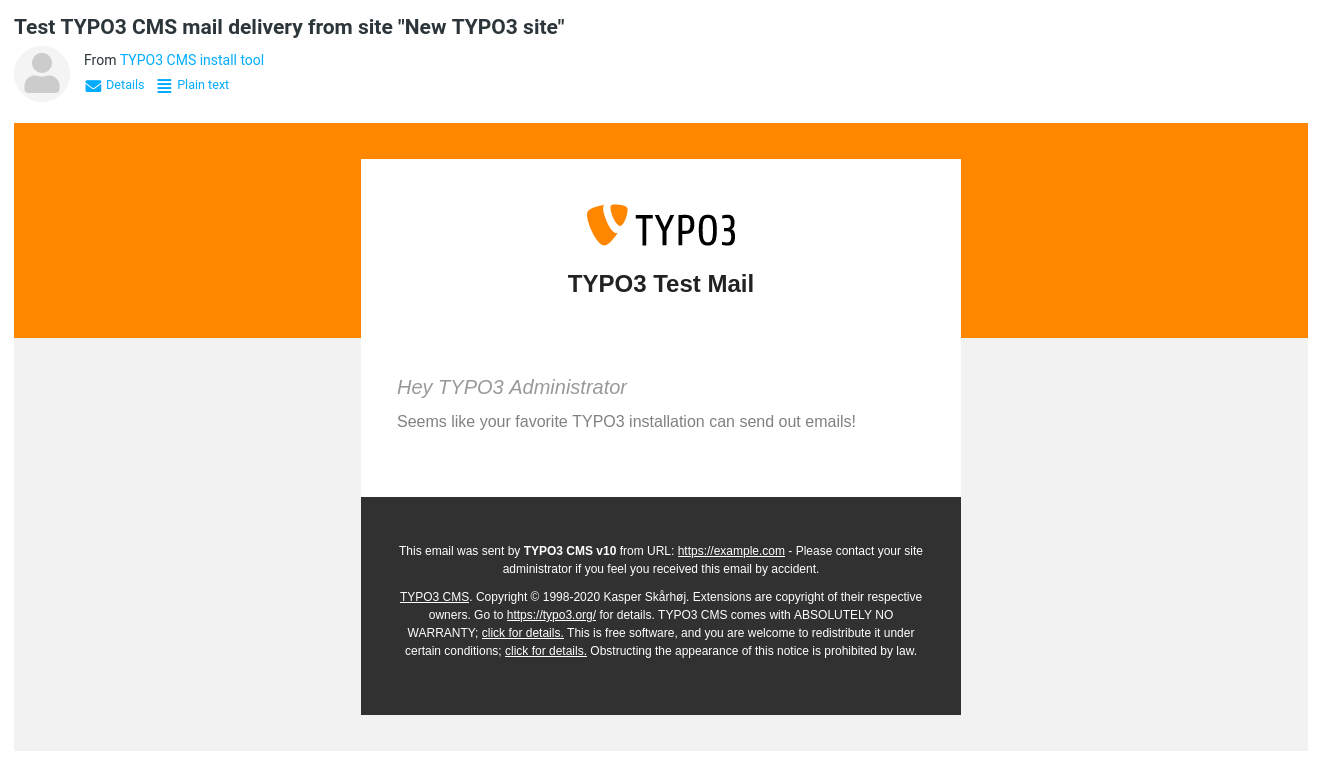
\includegraphics[width=0.8\linewidth]{ChangesForIntegrators/90266-FluidBasedTemplatedEmails.png}
	\end{figure}

\end{frame}

% ------------------------------------------------------------------------------
% Feature | 90203 | Make workspace available in TypoScript conditions

\begin{frame}[fragile]
	\frametitle{Änderungen für Integratoren}
	\framesubtitle{Workspaces und TypoScript}

	% decrease font size for code listing
	\lstset{basicstyle=\smaller\ttfamily}

	\begin{itemize}
		\item Es wurde eine neue Ausdruck-Sprachvariable hinzugefügt: \texttt{workspace}.
		\item Diese Variable kann verwendet werden, um einen gegebenen Begriff mit allgemeinen Workspace-Parametern abzugleichen.
		\item Derzeit werden die folgenden Parameter unterstützt:\newline
			\small
				\texttt{workspaceId}, \texttt{isLive}, and \texttt{isOffline}.
			\normalsize
		\item Zum Beispiel:

\vspace{-0.4cm}
\begin{lstlisting}
[workspace.workspaceId === 3]
  # Current workspace ID is 3
[end]
\end{lstlisting}

	\end{itemize}

\end{frame}

% ------------------------------------------------------------------------------
% Feature | 88962 | Re-implement old PIDupinRootline TypoScript condition

\begin{frame}[fragile]
	\frametitle{Änderungen für Integratoren}
	\framesubtitle{TypoScript}

	% decrease font size for code listing
	\lstset{basicstyle=\smaller\ttfamily}

	\begin{itemize}
		\item Die alte \texttt{PIDupinRootline} Bedingung wurde in TypoScript
			unter Verwendung der Symfony-Ausdruckssprache neu implementiert.
		\item Alte TypoScript-Bedingungssyntax:

\vspace{-0.4cm}
\begin{lstlisting}
[PIDupinRootline = 30]
  page.10.value = I'm on any subpage of page with UID 30.
[END]
\end{lstlisting}

		\item Neue TypoScript-Bedingungssyntax:

\vspace{-0.4cm}
\begin{lstlisting}
[30 in tree.rootLineParentIds]
  page.10.value = I'm on any subpage of page with UID 30.
[END]
\end{lstlisting}

	\end{itemize}

\end{frame}

% ------------------------------------------------------------------------------
% Feature | 90426 | Browser-native lazy loading for images

\begin{frame}[fragile]
	\frametitle{Änderungen für Integratoren}
	\framesubtitle{Lazy Loading für Bilder}

	% decrease font size for code listing
	\lstset{basicstyle=\smaller\ttfamily}

	\begin{itemize}
		\item Das HTML-Attribut \texttt{loading} kann nun für \texttt{<img>}-tags gesetzt werden.
		\item Browser, die diese Funktion unterstützen, laden diese Bilder erst, wenn sie sich im Ansichtsfenster befinden.
		\item Das Verhalten kann durch die folgende TypoScript-Konstante modifiziert werden:

\vspace{-0.4cm}
\begin{lstlisting}
styles.content.image.lazyLoading = lazy
\end{lstlisting}

		\item Gültige Werte sind: \texttt{lazy} (default), \texttt{eager}, und \texttt{auto}.
		\item Der Fluid \textit{Image-ViewHelper} unterstützt jetzt auch nachladen von Bildern bei Bedarf:

\vspace{-0.4cm}
\begin{lstlisting}
<f:image src="{fileObject}" treatIdAsReference="true"
  loading="lazy" />
\end{lstlisting}

	\end{itemize}

\end{frame}

% ------------------------------------------------------------------------------
% Important | 89869 | Change lockIP default to disabled for both frontend and backend

\begin{frame}[fragile]
	\frametitle{Änderungen für Integratoren}
	\framesubtitle{Standardwerte für \texttt{lockIP}/\texttt{lockIPv6}}

	% decrease font size for code listing
	\lstset{basicstyle=\smaller\ttfamily}

	\begin{itemize}
		\item Die Standardwerte für die \texttt{lockIP} Einstellungen wurden geändert.
		\item Die folgenden vier Systemvariablen sind jetzt standardmäßig \textbf{deaktiviert}:

			\begin{itemize}
				\item \texttt{[FE]['lockIP']}
				\item \texttt{[FE]['lockIPv6']}
				\item \texttt{[BE]['lockIP']}
				\item \texttt{[BE]['lockIPv6']}
			\end{itemize}

		\item Die alten Standardwerte ("\texttt{4}" für das Backend und "\texttt{2}" für das Frontend)
			verursachten Probleme z.B. bei Kunden mit IPv4- und IPv6-Adressen-Support.

	\end{itemize}

\end{frame}

% ------------------------------------------------------------------------------
% Feature | 90052 | Form YAML configuration available in configuration module

\begin{frame}[fragile]
	\frametitle{Änderungen für Integratoren}
	\framesubtitle{Form: YAML-Konfiguration}

	\begin{columns}[T]
		\begin{column}{.04\textwidth}
		\end{column}
		\begin{column}{.38\textwidth}

			Wenn die Systemerweiterung \texttt{EXT:form} installiert ist, kann die geparste YAML-Konfiguration
			unter \textbf{SYSTEM} $\rightarrow$ \textbf{Configuration} angezeigt werden.

			\vspace{0.2cm}

			Dies erfordert natürlich auch, dass Administratoren \texttt{EXT:lowlevel} aktivieren.

		\end{column}
		\begin{column}{.58\textwidth}
			\vspace{-0.3cm}
			\begin{figure}
				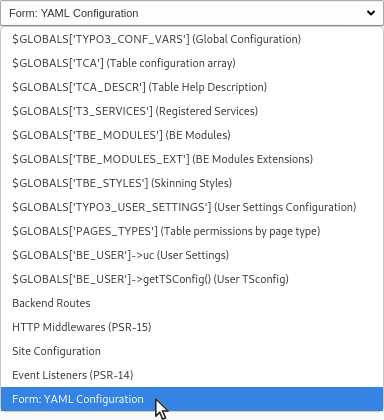
\includegraphics[width=0.70\linewidth]{ChangesForIntegrators/90052-AddYamlConfigurationToConfigurationModule.png}
			\end{figure}
		\end{column}
	\end{columns}

\end{frame}

% ------------------------------------------------------------------------------
% Feature | 88147 | Add possibility to configure the path to sitemap xslFile

\begin{frame}[fragile]
	\frametitle{Änderungen für Integratoren}
	\framesubtitle{SEO: \texttt{Sitemap.xsl}}

	% decrease font size for code listing
	\lstset{basicstyle=\tiny\ttfamily}

	\begin{itemize}
		\item Der Standardpfad zur Datei \texttt{Sitemap.xsl} der Systemerweiterung
			\texttt{EXT:seo} kann jetzt angepasst werden:

\vspace{-0.4cm}
\begin{lstlisting}
# Globally for all sitemaps:
plugin.tx_seo.config.xslFile = EXT:myext/Resources/Public/CSS/mySite.xsl

# For all sitemaps of a specific type:
plugin.tx_seo.config.<sitemapType>.sitemaps.xslFile = EXT:myext/Resources/Public/CSS/mySite.xsl

# For a specific sitemap:
plugin.tx_seo.config.<sitemapType>.sitemaps.<sitemap>.config.xslFile =
  EXT:myext/Resources/Public/CSS/mySite.xsl
\end{lstlisting}

		\item Der Standardpfad lautet:\newline
			\smaller
				\texttt{EXT:seo/Resources/Public/CSS/Sitemap.xsl}
			\normalsize

	\end{itemize}

\end{frame}

% ------------------------------------------------------------------------------
% Feature | 82062 | Progress for Reference Index update on CLI

\begin{frame}[fragile]
	\frametitle{Änderungen für Integratoren}
	\framesubtitle{Referenz-Index}

	% decrease font size for code listing
	\lstset{basicstyle=\tiny\ttfamily}

	\begin{itemize}
		\item Während der Aktualisierung des Referenz-Indexes werden für jede Datenbanktabelle Fortschrittbalken angezeigt.
	\end{itemize}

	\begin{figure}
		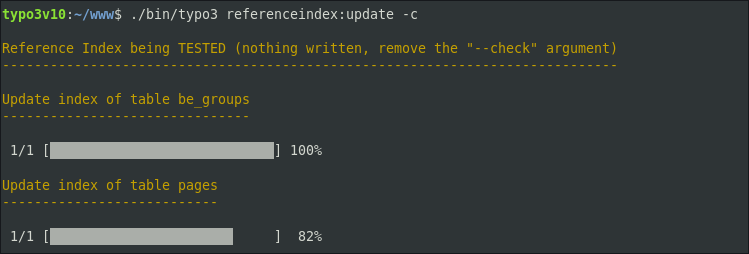
\includegraphics[width=0.85\linewidth]{ChangesForIntegrators/82062-ProgressForReferenceIndexUpdateOnCli.png}
	\end{figure}

\end{frame}

% ------------------------------------------------------------------------------
% Feature | 90425 | Add seo fields to info module

\begin{frame}[fragile]
	\frametitle{Änderungen für Integratoren}
	\framesubtitle{Info-Modul}

	\begin{itemize}
		\item SEO- und Social Media-Details wurden dem Info-Modul hinzugefügt:\newline
			\textbf{WEB} $\rightarrow$ \textbf{Info} $\rightarrow$ \textbf{Pagetree Overview}.
	\end{itemize}

	\begin{figure}
		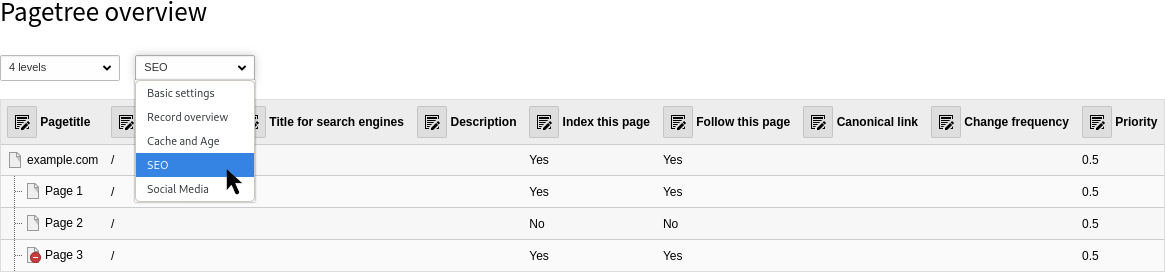
\includegraphics[width=0.85\linewidth]{ChangesForIntegrators/90425-AddSeoFieldsToInfoModule.png}
	\end{figure}

\end{frame}

% ------------------------------------------------------------------------------
% Feature | 59452 | scheduler:run command accepts multiple task options

\begin{frame}[fragile]
	\frametitle{Änderungen für Integratoren}
	\framesubtitle{Scheduler}

	% decrease font size for code listing
	\lstset{basicstyle=\tiny\ttfamily}

	\begin{itemize}
		\item Bei Verwendung der Option \texttt{-}\texttt{-}\texttt{task} können mehrere Aufgaben ausgeführt werden:
	\end{itemize}

	\begin{figure}
		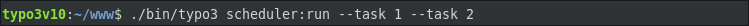
\includegraphics[width=0.85\linewidth]{ChangesForIntegrators/59452a-MultipleTasksInSchedulerCommand.png}
	\end{figure}

	\begin{itemize}
		\item Die ausführliche Ausgabe kann durch \texttt{-}\texttt{v} und \texttt{-}\texttt{vv} aktiviert werden:
	\end{itemize}

	\begin{figure}
		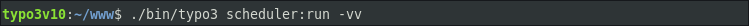
\includegraphics[width=0.85\linewidth]{ChangesForIntegrators/59452b-MultipleTasksInSchedulerCommand.png}
	\end{figure}

\end{frame}

% ------------------------------------------------------------------------------
% Feature | 90298 | Improve user info in BE User module

\begin{frame}[fragile]
	\frametitle{Änderungen für Integratoren}
	\framesubtitle{Backend-Benutzer-Modul}

	\begin{itemize}
		\item Eine neue Detailansicht der BE-Benutzereinträge zeigt alle relevanten Daten an.
		\item Der Funktion wurden zusätzliche Felder hinzugefügt, um Benutzer zu vergleichen.
		\item Diese Funktion berücksichtigt jetzt auch Untergruppen.
		\item Die Benutzerschnittstelle des Moduls wird weiter angepasst und optimiert werden.
		\item Diese Änderungen erleichtern Integratoren/Administratoren die 
			Überprüfung und den Vergleich von Benutzerberechtigungen, ohne zum Benutzer zu wechseln.
	\end{itemize}

\end{frame}

% ------------------------------------------------------------------------------
% Feature | 89894 | Separate system extensions from 3rd-party extensions visually

\begin{frame}[fragile]
	\frametitle{Backend User Interface}
	\framesubtitle{Extension Manager}

	System und Third Party Erweiterungen können jetzt im Extension Manager getrennt aufgeführt werden.

	\begin{figure}
		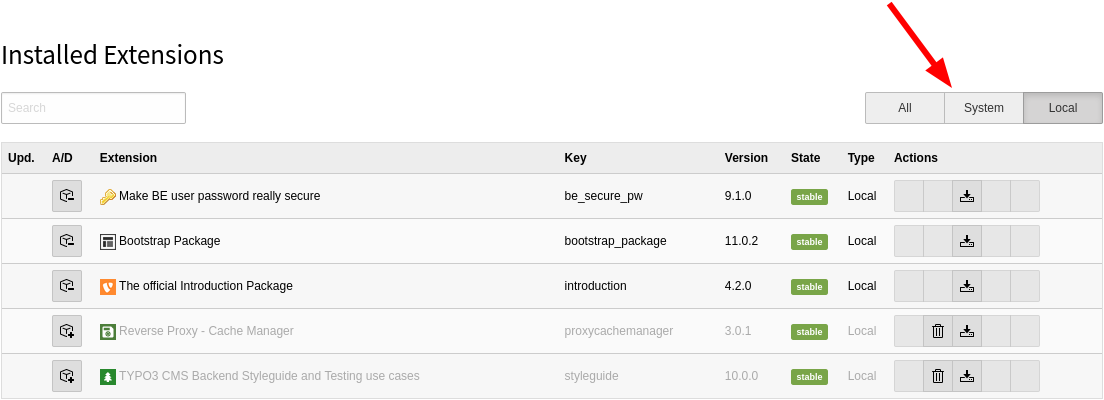
\includegraphics[width=0.9\linewidth]{BackendUserInterface/89894-SeparateSystemExtensionsFrom3rdPartyExtensionsVisually.png}
	\end{figure}

\end{frame}

% ------------------------------------------------------------------------------
% Feature | 90136 | Show application context in the Environment module

\begin{frame}[fragile]
	\frametitle{Änderungen für Integratoren}
	\framesubtitle{Environment Übersicht}

	Der aktuelle Anwendungskontext wird nun im Environment-Modul angezeigt:\newline
	\textbf{ADMIN TOOLS} $\rightarrow$ \textbf{Environment} $\rightarrow$ \textbf{Environment Overview}.

	\begin{figure}
		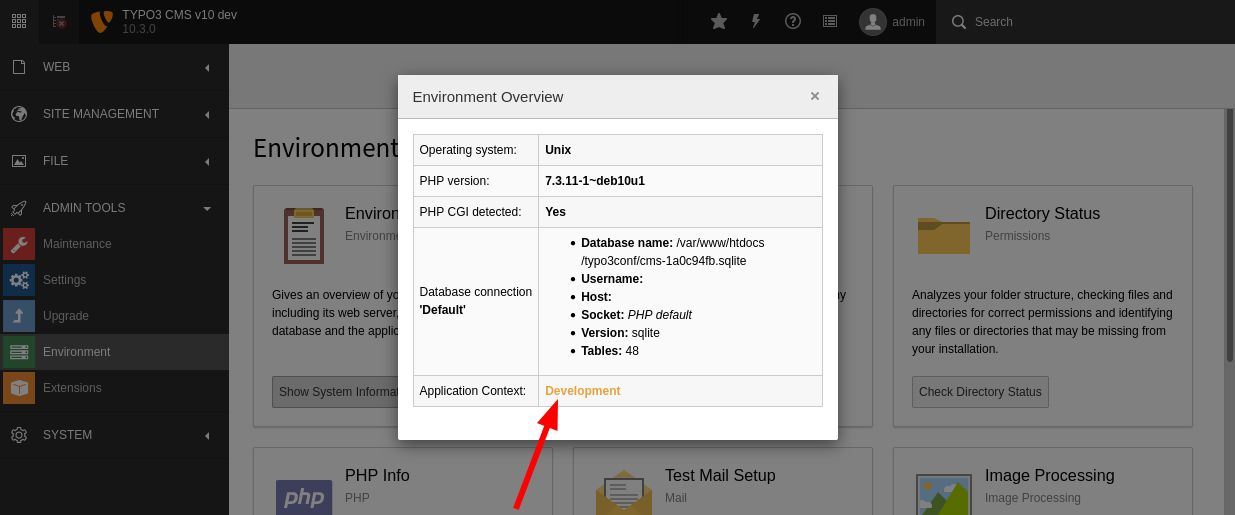
\includegraphics[width=0.9\linewidth]{ChangesForIntegrators/90136-ShowApplicationContextInTheEnvironmentModule.png}
	\end{figure}

\end{frame}

% ------------------------------------------------------------------------------
% Task | 89844 | Improve visual appearance of feature toggles

\begin{frame}[fragile]
	\frametitle{Änderungen für Integratoren}
	\framesubtitle{Feature-Schalter}

	Das Erscheinungsbild des Feature-Schalters wurde verbessert:
	\newline\newline
	\smaller\textbf{TYPO3 < 10.3}\tabto{6cm}\textbf{TYPO3 >= 10.3}\normalsize

	\begin{figure}
		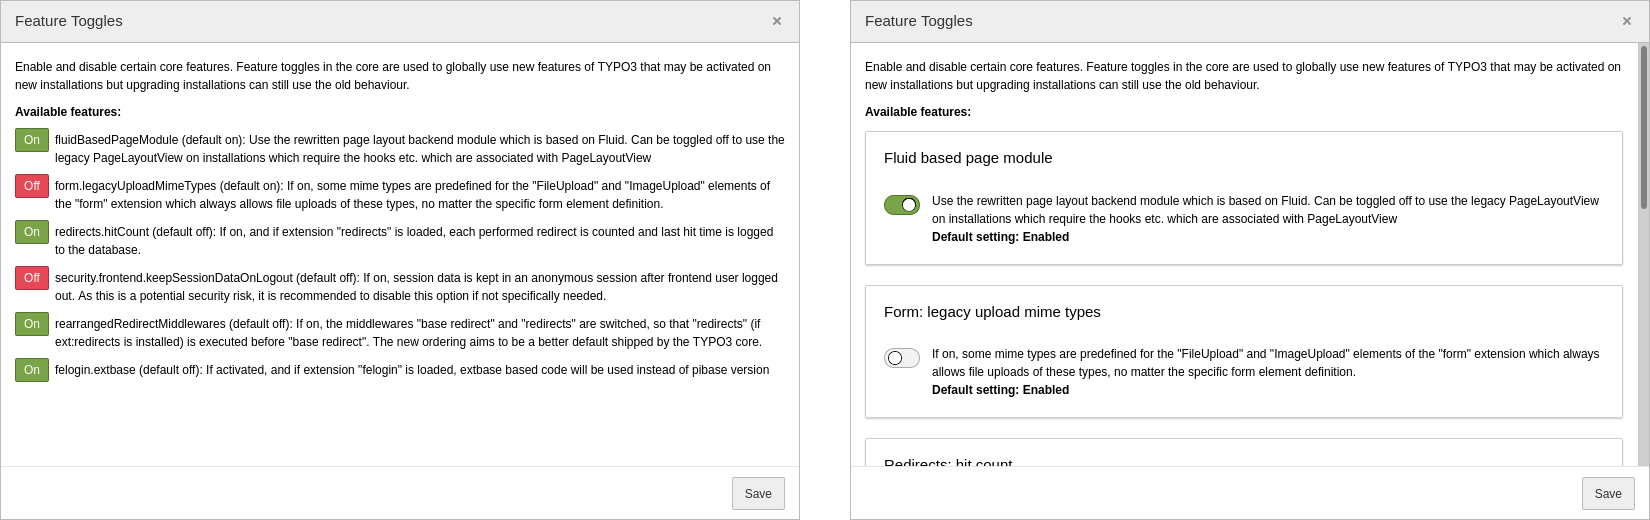
\includegraphics[width=1\linewidth]{ChangesForIntegrators/89844-ImproveVisualAppearanceOfFeatureToggles.png}
	\end{figure}

\end{frame}

% ------------------------------------------------------------------------------
% Feature | 89513 | Provide password recovery for backend users
%
%\begin{frame}[fragile]
%	\frametitle{Changes for Integrators}
%	\framesubtitle{Password Recovery Email}
%
%	\begin{itemize}
%
%		\item Password resets for backend users are only valid for 4 hours.\newline
%			This time limit is not configurable.
%		\item The function can optionally be disabled for all users or for admin users only to strengthen security.
%		\item If users share one email address, an alternative email text is used.
%		\item TCA field \texttt{be\_users.email} must not be set to \texttt{eval=email}.
%
%		\item The function only works for users, who:
%			\begin{itemize}
%				\item have an email address set,
%				\item have a password set, and
%				\item are not disabled/deleted.
%			\end{itemize}
%
%	\end{itemize}
%
%\end{frame}
%
% ------------------------------------------------------------------------------
